\documentclass[8pt]{beamer}
\usetheme{Madrid}
\usecolortheme{default}
\usepackage{amsmath, amssymb, graphicx, array, multirow, booktabs, xcolor, tikz}
\usetikzlibrary{shapes,arrows,positioning,fit,backgrounds}

% Compact font settings
\setbeamerfont{title}{size=\Large}
\setbeamerfont{subtitle}{size=\small}
\setbeamerfont{author}{size=\scriptsize}
\setbeamerfont{date}{size=\scriptsize}
\setbeamerfont{frametitle}{size=\large}
\setbeamerfont{framesubtitle}{size=\normalsize}
\setbeamerfont{enumerate item}{size=\footnotesize}
\setbeamerfont{itemize item}{size=\footnotesize}
\setbeamerfont{block title}{size=\footnotesize}

% Compact spacing
\setlength{\itemsep}{0.08ex}
\setlength{\parskip}{0.08ex}
\setlength{\leftmargini}{0.3cm}
\setbeamersize{text margin left=3mm, text margin right=3mm}
\addtobeamertemplate{frame begin}{\vspace{-0.4cm}}{}

% Colors
\definecolor{blue}{RGB}{0,0,255}
\definecolor{red}{RGB}{255,0,0}
\definecolor{green}{RGB}{0,128,0}
\definecolor{orange}{RGB}{255,165,0}
\definecolor{purple}{RGB}{128,0,128}
\definecolor{gray}{RGB}{128,128,128}

\title{Reinforcement Learning - Part 2}
\subtitle{Deep RL, DQN, Policy Methods, MDP, Bellman, Advanced Topics}
\author{GARP RAI Exam Preparation}
\date{}

\begin{document}

\begin{frame}
\titlepage
\end{frame}

% ============================================================
% SLIDES 51-60: DEEP RL & DQN
% ============================================================

\begin{frame}{TUTORIAL OVERVIEW - Part 2}
\fontsize{7}{8}\selectfont
\textbf{What You Will Learn in Part 2:}

\vspace{0.2cm}
\begin{tabular}{|p{2.5cm}|p{5.5cm}|}
\hline
\textcolor{blue}{Topic} & \textcolor{blue}{Key Concepts Covered} \\
\hline
5. Deep RL \& DQN & Neural Networks, Experience Replay, Target Networks \\
\hline
6. Policy Methods & Value-based vs Policy-based, Actor-Critic, Continuous Actions \\
\hline
7. MDP \& Bellman & Markov Property, Dynamic Programming, Optimality Equations \\
\hline
8. Advanced Topics & RLHF, AlphaGo, Model-Based RL, Continuous RL \\
\hline
\end{tabular}

\vspace{0.2cm}
\textbf{Key to Success:} Understand the \textcolor{blue}{"exploration vs exploitation"} trade-off!
\end{frame}

\begin{frame}{Deep RL - Introduction}
\fontsize{6.5}{7.5}\selectfont
\textcolor{blue}{\textbf{Deep Reinforcement Learning - Scaling RL}}

\textbf{The Problem with Tabular Methods:}
\begin{itemize}
\item Q-table stores Q(s,a) for every state-action pair
\item Number of states can be \textcolor{red}{enormous} (or infinite)
\item Example: Atari games have $10^{50}$ possible states!
\item Self-driving cars have continuous state spaces
\end{itemize}

\textbf{The Solution: Deep RL}
\begin{itemize}
\item Use \textcolor{blue}{neural networks} to approximate Q(s,a)
\item $Q(s,a) \approx Q(s,a; \theta)$ where $\theta$ = network weights
\item Neural network takes state as input, outputs Q-values for all actions
\end{itemize}

\textbf{Why Neural Networks?}
\begin{enumerate}
\item \textcolor{blue}{Generalization}: Similar states get similar Q-values
\item \textcolor{blue}{Compact representation}: No need to store all states
\item \textcolor{blue}{Continuous spaces}: Can handle continuous state inputs
\end{enumerate}

\textbf{Deep RL Architecture:}
\begin{center}
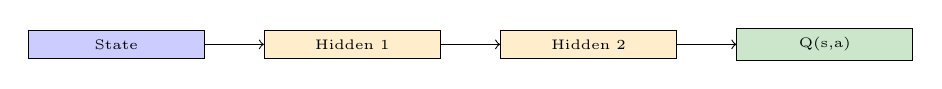
\begin{tikzpicture}[scale=0.4, every node/.style={font=\tiny}]
\node[draw, rectangle, fill=blue!20, text width=2cm, align=center] (state) {State};
\node[draw, rectangle, fill=orange!20, text width=2cm, align=center] (hidden1) [right of=state, xshift=2cm] {Hidden 1};
\node[draw, rectangle, fill=orange!20, text width=2cm, align=center] (hidden2) [right of=hidden1, xshift=2cm] {Hidden 2};
\node[draw, rectangle, fill=green!20, text width=2cm, align=center] (output) [right of=hidden2, xshift=2cm] {Q(s,a)};
\draw[->] (state) -- (hidden1);
\draw[->] (hidden1) -- (hidden2);
\draw[->] (hidden2) -- (output);
\end{tikzpicture}
\end{center}

\textcolor{red}{\textbf{Exam Trap:}} Deep RL is needed when state spaces are too large for tables!
\end{frame}

\begin{frame}{DQN - Introduction}
\fontsize{6.5}{7.5}\selectfont
\textcolor{blue}{\textbf{Deep Q-Network - The Breakthrough}}

\textbf{What is DQN?}
\begin{itemize}
\item Combines Q-learning with \textcolor{blue}{deep neural networks}
\item Developed by DeepMind (2015)
\item Achieved human-level performance on Atari games
\end{itemize}

\textbf{Three Key Innovations:}
\begin{enumerate}
\item \textcolor{blue}{Experience Replay}: Store experiences and sample randomly
\item \textcolor{blue}{Target Network}: Separate network for stable targets
\item \textcolor{blue}{$\epsilon$-Greedy}: For exploration
\end{enumerate}

\textbf{DQN Architecture:}
\begin{center}
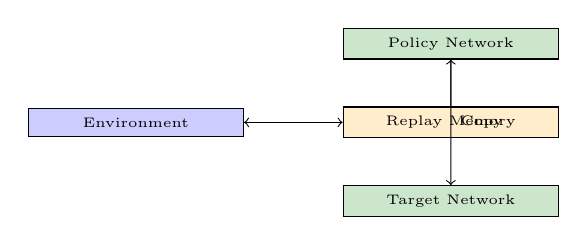
\begin{tikzpicture}[scale=0.4, every node/.style={font=\tiny}]
\node[draw, rectangle, fill=blue!20, text width=2.5cm, align=center] (env) {Environment};
\node[draw, rectangle, fill=orange!20, text width=2.5cm, align=center] (replay) [right of=env, xshift=3cm] {Replay Memory};
\node[draw, rectangle, fill=green!20, text width=2.5cm, align=center] (policy) [above of=replay] {Policy Network};
\node[draw, rectangle, fill=green!20, text width=2.5cm, align=center] (target) [below of=replay] {Target Network};
\draw[<->] (env) -- (replay);
\draw[->] (replay) -- (policy);
\draw[->] (policy) -- (target) node[midway,right] {Copy};
\end{tikzpicture}
\end{center}

\textbf{How DQN Works:}
\begin{enumerate}
\item Interact with environment, store experiences
\item Sample random mini-batch from replay memory
\item Update policy network using TD target from target network
\item Periodically copy policy network weights to target network
\end{enumerate}

\textcolor{red}{\textbf{Exam Trap:}} DQN's success comes from experience replay and target network!
\end{frame}

\begin{frame}{DQN - Experience Replay}
\fontsize{6.5}{7.5}\selectfont
\textcolor{blue}{\textbf{Experience Replay - Why It's Critical}}

\textbf{The Problem:}
\begin{itemize}
\item Consecutive experiences in RL are \textcolor{red}{highly correlated}
\item Example: In a game, consecutive frames are nearly identical
\item Correlated data breaks the i.i.d. assumption of supervised learning
\end{itemize}

\textbf{The Solution: Experience Replay}
\begin{enumerate}
\item Store experiences $(s, a, r, s')$ in a \textcolor{blue}{replay memory}
\item During training, sample \textcolor{blue}{random mini-batches} from memory
\item This breaks temporal correlation
\end{enumerate}

\textbf{Why Random Sampling?}
\begin{itemize}
\item Reduces correlation between samples
\item Makes learning more stable
\item Reuses experiences multiple times (more efficient)
\end{itemize}

\textbf{Replay Memory Structure:}
\begin{itemize}
\item Fixed size (e.g., 1,000,000 experiences)
\item Oldest experiences are discarded (FIFO)
\item Random sampling (uniform or prioritized)
\end{itemize}

\textbf{Benefits:}
\begin{enumerate}
\item \textcolor{green}{Stable learning}: Breaks correlations
\item \textcolor{green}{Efficient}: Reuses experiences
\item \textcolor{green}{Reduces variance}: Averaging over random samples
\end{enumerate}

\textbf{Prioritized Experience Replay:}
\begin{itemize}
\item Sample experiences with \textcolor{blue}{higher TD error} more often
\item Focuses on experiences that are most "surprising"
\end{itemize}

\textcolor{red}{\textbf{Exam Trap:}} Experience replay breaks temporal correlation!
\end{frame}

\begin{frame}{DQN - Target Network}
\fontsize{6.5}{7.5}\selectfont
\textcolor{blue}{\textbf{Target Network - Stabilizing the Moving Target}}

\textbf{The Problem:}
\begin{itemize}
\item Q-learning uses $R + \gamma \max_{a'} Q(s',a')$ as target
\item But $Q(s',a')$ is the \textcolor{red}{same network} being updated!
\item This creates a \textcolor{red}{"chasing the moving target"} problem
\end{itemize}

\textbf{The Solution: Target Network}
\begin{itemize}
\item Use a \textcolor{blue}{separate network} for the target
\item Target network weights: $\theta^-$
\item Policy network weights: $\theta$
\end{itemize}

\textbf{How It Works:}
\begin{enumerate}
\item Policy network: Used to select actions ($\epsilon$-greedy)
\item Target network: Used to compute TD target
\item Update policy network: $L = (Q(s,a;\theta) - (R + \gamma \max_{a'} Q(s',a';\theta^-)))^2$
\item Periodically copy: $\theta^- \leftarrow \theta$
\end{enumerate}

\textbf{Update Frequency:}
\begin{itemize}
\item Typical: Copy every \textcolor{blue}{500} steps
\item Too frequent: Target moves too fast (unstable)
\item Too infrequent: Target is outdated (slow learning)
\end{itemize}

\textbf{Benefits:}
\begin{enumerate}
\item \textcolor{green}{Stable targets}: Target doesn't change every step
\item \textcolor{green}{More stable learning}: Reduces oscillations
\item \textcolor{green}{Convergence}: Helps converge to optimal policy
\end{enumerate}

\textcolor{red}{\textbf{Exam Trap:}} Target network is updated periodically!
\end{frame}

\begin{frame}{DQN - Loss Function}
\fontsize{6.5}{7.5}\selectfont
\textcolor{blue}{\textbf{DQN Loss Function and Training}}

\textbf{Loss Function (MSE):}
\[
L(\theta) = \mathbb{E}_{(s,a,r,s') \sim U(D)}[(Q(s,a;\theta) - (r + \gamma \max_{a'} Q(s',a';\theta^-)))^2]
\]

\textbf{Components:}
\begin{itemize}
\item $Q(s,a;\theta)$: Policy network prediction
\item $r + \gamma \max_{a'} Q(s',a';\theta^-)$: TD target from target network
\item $U(D)$: Uniform random sampling from replay memory
\end{itemize}

\textbf{Training Process:}
\begin{enumerate}
\item Sample random mini-batch from replay memory
\item For each experience:
\begin{enumerate}
\item Compute target: $y = r + \gamma \max_{a'} Q(s',a';\theta^-)$
\item Compute prediction: $Q(s,a;\theta)$
\item Compute loss: $(y - Q(s,a;\theta))^2$
\end{enumerate}
\item Average loss over mini-batch
\item Backpropagate and update $\theta$
\end{enumerate}

\textbf{Gradient Update:}
\[
\theta \leftarrow \theta - \alpha \nabla_\theta L(\theta)
\]

\textbf{Hyperparameters:}
\begin{itemize}
\item Learning rate $\alpha$: 0.001 (typical)
\item Mini-batch size: 32 or 64
\item Replay memory size: 1,000,000
\end{itemize}

\textcolor{red}{\textbf{Exam Trap:}} DQN loss is MSE between policy and target networks!
\end{frame}

\begin{frame}{DQN - Training Algorithm}
\fontsize{6.5}{7.5}\selectfont
\textcolor{blue}{\textbf{DQN Training - Step-by-Step Process}}

\textbf{Algorithm:}
\begin{enumerate}
\item \textcolor{blue}{Initialize:}
\begin{itemize}
\item Policy network $Q(s,a;\theta)$ with random weights
\item Target network $Q(s,a;\theta^-)$ with same weights
\item Replay memory $D$ of capacity $N$
\end{itemize}

\item \textcolor{blue}{For each episode:}
\begin{enumerate}
\item Initialize state $s$
\item For each step:
\begin{enumerate}
\item With probability $\epsilon$: Choose random action (explore)
\item Otherwise: Choose $a = \arg\max_a Q(s,a;\theta)$ (exploit)
\item Take action $a$, observe reward $r$ and next state $s'$
\item Store $(s,a,r,s')$ in $D$
\item Sample random mini-batch from $D$
\item Compute loss and update $\theta$
\item Periodically update $\theta^- \leftarrow \theta$
\item Set $s \leftarrow s'$
\end{enumerate}
\end{enumerate}
\end{enumerate}

\textbf{$\epsilon$ Decay in DQN:}
\begin{itemize}
\item Start with $\epsilon = 1.0$ (pure exploration)
\item Decay to $\epsilon = 0.01$ (mostly exploitation)
\item Linear decay over first 1,000,000 steps
\end{itemize}

\textbf{Stopping Criteria:}
\begin{itemize}
\item Maximum number of steps reached
\item No improvement in Q-values
\item Episode reward converges
\end{itemize}

\textcolor{red}{\textbf{Exam Trap:}} DQN has two networks: policy and target!
\end{frame}

\begin{frame}{DQN - Convergence and Stability}
\fontsize{6.5}{7.5}\selectfont
\textcolor{blue}{\textbf{DQN - Ensuring Stable Learning}}

\textbf{Challenges in Deep RL:}
\begin{enumerate}
\item \textcolor{red}{Non-stationarity}: The target distribution changes
\item \textcolor{red}{Correlation}: Consecutive samples are correlated
\item \textcolor{red}{Divergence}: Q-learning with function approximation can diverge
\end{enumerate}

\textbf{DQN Solutions:}
\begin{enumerate}
\item \textcolor{blue}{Experience Replay}: Breaks correlation
\item \textcolor{blue}{Target Network}: Stabilizes targets
\item \textcolor{blue}{Gradient Clipping}: Prevents exploding gradients
\item \textcolor{blue}{Frame Stacking}: Gives temporal context
\end{enumerate}

\textbf{Gradient Clipping:}
\begin{itemize}
\item Clip gradients to a maximum value
\item Prevents very large updates
\item Common threshold: 1.0 or 10.0
\end{itemize}

\textbf{Frame Stacking (for Atari):}
\begin{itemize}
\item Stack last 4 frames
\item Provides temporal information (motion)
\item Input: 84x84x4 image
\end{itemize}

\textbf{Double DQN:}
\begin{itemize}
\item Uses target network for action selection too
\item Reduces overestimation bias
\item $y = r + \gamma Q(s', \arg\max_{a'} Q(s',a';\theta); \theta^-)$
\end{itemize}

\textbf{Dueling DQN:}
\begin{itemize}
\item Separate value and advantage streams
\item Better estimate of state values
\item $Q(s,a) = V(s) + (A(s,a) - \frac{1}{|\mathcal{A}|}\sum_{a'} A(s,a'))$
\end{itemize}

\textcolor{red}{\textbf{Exam Trap:}} DQN can be unstable - use experience replay and target networks!
\end{frame}

\begin{frame}{DQN - Extensions}
\fontsize{6.5}{7.5}\selectfont
\textcolor{blue}{\textbf{DQN Extensions - Making It Better}}

\textbf{Double DQN:}
\begin{itemize}
\item Uses target network for action selection too
\item Reduces overestimation bias
\item $y = r + \gamma Q(s', \arg\max_{a'} Q(s',a';\theta); \theta^-)$
\end{itemize}

\textbf{Dueling DQN:}
\begin{itemize}
\item Separate value and advantage streams
\item Better estimate of state values
\item $Q(s,a) = V(s) + (A(s,a) - \frac{1}{|\mathcal{A}|}\sum_{a'} A(s,a'))$
\end{itemize}

\textbf{Prioritized Experience Replay:}
\begin{itemize}
\item Sample experiences with higher TD error more often
\item Focuses on most "surprising" experiences
\item Can improve learning efficiency
\end{itemize}

\textbf{Rainbow:}
\begin{itemize}
\item Combines multiple DQN improvements:
\begin{itemize}
\item Double DQN
\item Dueling DQN
\item Prioritized Experience Replay
\item Multi-step learning
\item Distributional RL
\item Noisy Nets
\end{itemize}
\item State-of-the-art performance
\end{itemize}

\textcolor{red}{\textbf{Exam Trap:}} Double DQN and Dueling DQN are key extensions!
\end{frame}

\begin{frame}{DQN - Advantages and Limitations}
\fontsize{6.5}{7.5}\selectfont
\textcolor{blue}{\textbf{DQN - Pros, Cons, and When to Use}}

\textbf{Advantages:}
\begin{enumerate}
\item \textcolor{green}{Handles large state spaces} - neural networks generalize
\item \textcolor{green}{State-of-the-art on many games}
\item \textcolor{green}{Can learn directly from raw pixels}
\item \textcolor{green}{Combines deep learning with RL}
\end{enumerate}

\textbf{Limitations:}
\begin{enumerate}
\item \textcolor{red}{Computationally expensive} - training can take days
\item \textcolor{red}{Requires many samples} - millions of interactions
\item \textcolor{red}{Limited to discrete action spaces} - outputs Q-values per action
\item \textcolor{red}{Can be unstable} - hyperparameter sensitive
\end{enumerate}

\textbf{When to Use DQN:}
\begin{itemize}
\item Large discrete action spaces
\item High-dimensional state spaces (images)
\item When you have computational resources
\item When samples are plentiful
\end{itemize}

\textbf{When NOT to Use DQN:}
\begin{itemize}
\item Small state spaces (tabular methods are better)
\item Continuous action spaces (use policy-based methods)
\item When samples are expensive
\end{itemize}

\textcolor{red}{\textbf{Exam Trap:}} DQN is only for discrete action spaces!
\end{frame}

\begin{frame}{DQN - Summary}
\fontsize{6.5}{7.5}\selectfont
\textcolor{blue}{\textbf{DQN - Complete Summary}}

\textbf{Key Concepts:}
\begin{enumerate}
\item \textcolor{blue}{DQN = Q-Learning + Deep Neural Networks}
\begin{itemize}
\item Replaces Q-table with neural network
\item Input: state; Output: Q-values for all actions
\end{itemize}

\item \textcolor{blue}{Three Key Innovations:}
\begin{enumerate}
\item \textcolor{blue}{Experience Replay}: Random sampling breaks correlation
\item \textcolor{blue}{Target Network}: Separate network for stable targets
\item \textcolor{blue}{$\epsilon$-Greedy}: Exploration/exploitation balance
\end{enumerate}

\item \textcolor{blue}{Loss Function:}
\[
L = \mathbb{E}[(Q(s,a;\theta) - (R + \gamma \max_{a'} Q(s',a';\theta^-)))^2]
\]

\item \textcolor{blue}{Update Steps:}
\begin{enumerate}
\item Sample mini-batch from replay memory
\item Compute targets using target network
\item Update policy network
\item Periodically copy weights to target network
\end{enumerate}

\item \textcolor{blue}{Limitations:}
\begin{itemize}
\item Discrete actions only
\item Computationally expensive
\item Sample inefficient
\end{itemize}
\end{enumerate}

\textcolor{red}{\textbf{Exam Success:}} Remember DQN's three key innovations!
\end{frame}

% ============================================================
% SLIDES 61-70: POLICY METHODS
% ============================================================

\begin{frame}{Policy Methods - Introduction}
\fontsize{6.5}{7.5}\selectfont
\textcolor{blue}{\textbf{Policy-Based Methods - Learning Strategy Directly}}

\textbf{Value-Based vs Policy-Based:}
\begin{tabular}{|c|c|}
\hline
Value-Based & Policy-Based \\
\hline
Learn Q(s,a) & Learn $\pi(a|s)$ directly \\
\hline
Derive policy from Q & Policy is the output \\
\hline
Q-learning, SARSA & Policy Gradient \\
\hline
Discrete actions only & Continuous actions possible \\
\hline
\end{tabular}

\textbf{Policy Representation:}
\begin{itemize}
\item Policy parameterized: $\pi_\theta(a|s)$
\item $\theta$ = parameters (neural network weights)
\item Neural network takes state $s$ as input
\item Output: probability distribution over actions
\end{itemize}

\textbf{Policy Gradient:}
\begin{itemize}
\item Optimize $\theta$ to maximize expected reward
\item Gradient ascent on $J(\theta) = E_\pi[\sum R]$
\item Update: $\theta \leftarrow \theta + \alpha \nabla_\theta J(\theta)$
\end{itemize}

\textbf{Why Policy Methods?}
\begin{enumerate}
\item \textcolor{blue}{Continuous action spaces}: Can output continuous actions
\item \textcolor{blue}{Stochastic policies}: Natural for partial observability
\item \textcolor{blue}{Better convergence}: Guaranteed to converge to local optimum
\end{enumerate}

\textcolor{red}{\textbf{Exam Trap:}} Policy methods are preferred for continuous action spaces!
\end{frame}

\begin{frame}{REINFORCE Algorithm}
\fontsize{6.5}{7.5}\selectfont
\textcolor{blue}{\textbf{REINFORCE - Monte Carlo Policy Gradient}}

\textbf{The REINFORCE Algorithm:}
\begin{itemize}
\item Monte Carlo policy gradient method
\item Updates after complete episodes
\item Uses the actual return $G_t$
\end{itemize}

\textbf{Update Formula:}
\[
\theta \leftarrow \theta + \alpha \gamma^t G_t \nabla_\theta \log \pi_\theta(a_t|s_t)
\]

\textbf{Intuition:}
\begin{itemize}
\item If $G_t$ is positive (good outcome), increase probability of action
\item If $G_t$ is negative (bad outcome), decrease probability of action
\item The gradient $\nabla_\theta \log \pi_\theta$ points in the direction to increase the action's probability
\end{itemize}

\textbf{Algorithm Steps:}
\begin{enumerate}
\item Initialize policy parameters $\theta$
\item For each episode:
\begin{enumerate}
\item Generate episode: $s_0, a_0, r_1, s_1, ..., s_T$
\item For each step $t$:
\begin{enumerate}
\item Compute $G_t = \sum_{k=t+1}^T \gamma^{k-t-1} r_k$
\item Update $\theta \leftarrow \theta + \alpha \gamma^t G_t \nabla_\theta \log \pi_\theta(a_t|s_t)$
\end{enumerate}
\end{enumerate}
\end{enumerate}

\textbf{Advantages:}
\begin{itemize}
\item Simple to implement
\item Theoretically sound
\item Works for continuous actions
\end{itemize}

\textbf{Disadvantages:}
\begin{itemize}
\item High variance (like MC)
\item Requires complete episodes
\item Slow convergence
\end{itemize}

\textcolor{red}{\textbf{Exam Trap:}} REINFORCE is MC-based with high variance!
\end{frame}

\begin{frame}{Actor-Critic Methods}
\fontsize{6.5}{7.5}\selectfont
\textcolor{blue}{\textbf{Actor-Critic - The Best of Both Worlds}}

\textbf{What is Actor-Critic?}
\begin{itemize}
\item Combines \textcolor{blue}{value-based} and \textcolor{blue}{policy-based} methods
\item \textcolor{blue}{Actor}: Learns the policy (policy-based)
\item \textcolor{blue}{Critic}: Learns the value function (value-based)
\item Critic evaluates actor's actions
\end{itemize}

\textbf{Architecture:}
\begin{center}
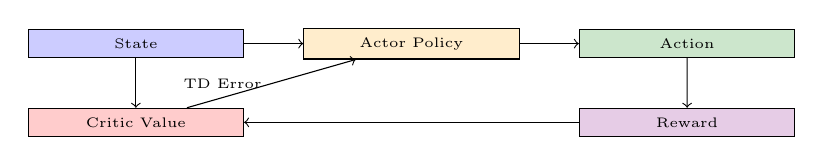
\begin{tikzpicture}[scale=0.4, every node/.style={font=\tiny}]
\node[draw, rectangle, fill=blue!20, text width=2.5cm, align=center] (state) {State};
\node[draw, rectangle, fill=orange!20, text width=2.5cm, align=center] (actor) [right of=state, xshift=2.5cm] {Actor Policy};
\node[draw, rectangle, fill=green!20, text width=2.5cm, align=center] (action) [right of=actor, xshift=2.5cm] {Action};
\node[draw, rectangle, fill=red!20, text width=2.5cm, align=center] (critic) [below of=state] {Critic Value};
\node[draw, rectangle, fill=purple!20, text width=2.5cm, align=center] (reward) [below of=action] {Reward};
\draw[->] (state) -- (actor);
\draw[->] (state) -- (critic);
\draw[->] (actor) -- (action);
\draw[->] (action) -- (reward);
\draw[->] (reward) -- (critic);
\draw[->] (critic) -- (actor) node[midway,left] {TD Error};
\end{tikzpicture}
\end{center}

\textbf{How It Works:}
\begin{enumerate}
\item Actor takes action based on current policy
\item Critic evaluates the action (TD error)
\item TD error: $\delta = R + \gamma V(s') - V(s)$
\item If $\delta > 0$: Action was better than expected $\rightarrow$ increase probability
\item If $\delta < 0$: Action was worse than expected $\rightarrow$ decrease probability
\end{enumerate}

\textbf{Advantages:}
\begin{enumerate}
\item \textcolor{green}{Lower variance} than policy gradient
\item \textcolor{green}{Can learn online} (TD-based)
\item \textcolor{green}{Continuous action spaces} (policy-based)
\end{enumerate}

\textcolor{red}{\textbf{Exam Trap:}} Actor-Critic combines policy (actor) and value (critic)!
\end{frame}

\begin{frame}{Policy Methods - Summary}
\fontsize{6.5}{7.5}\selectfont
\textcolor{blue}{\textbf{Policy Methods - Complete Summary}}

\textbf{Key Concepts:}
\begin{enumerate}
\item \textcolor{blue}{Policy-Based Methods:}
\begin{itemize}
\item Learn policy $\pi_\theta(a|s)$ directly
\item Output: action (or probability distribution)
\item Better for continuous action spaces
\end{itemize}

\item \textcolor{blue}{Value-Based Methods:}
\begin{itemize}
\item Learn Q(s,a) or V(s)
\item Output: value estimates
\item Derive policy from values
\item Better for discrete action spaces
\end{itemize}

\item \textcolor{blue}{REINFORCE:}
\begin{itemize}
\item MC policy gradient
\item High variance
\item Requires complete episodes
\end{itemize}

\item \textcolor{blue}{Actor-Critic:}
\begin{itemize}
\item Actor: Policy
\item Critic: Value function
\item Lower variance
\item Can learn online
\end{itemize}

\item \textcolor{blue}{Advantages of Policy Methods:}
\begin{itemize}
\item Continuous actions
\item Stochastic policies
\item Better convergence
\end{itemize}

\item \textcolor{blue}{Disadvantages of Policy Methods:}
\begin{itemize}
\item Slow convergence
\item Local optima
\item Sample inefficient
\end{itemize}
\end{enumerate}

\textcolor{red}{\textbf{Exam Success:}} Choose between value-based and policy-based based on action space!
\end{frame}

% ============================================================
% SLIDES 71-80: MDP & BELLMAN
% ============================================================

\begin{frame}{MDP - Formal Definition}
\fontsize{6.5}{7.5}\selectfont
\textcolor{blue}{\textbf{Markov Decision Processes - The RL Framework}}

\textbf{What is an MDP?}
\begin{itemize}
\item Mathematical framework for modeling decision-making
\item Defined by: States, Actions, Transition Probabilities, Rewards
\item Assumes the \textcolor{blue}{Markov property}
\end{itemize}

\textbf{MDP Components:}
\begin{enumerate}
\item \textcolor{blue}{States ($S$)}: Set of all possible states
\item \textcolor{blue}{Actions ($A$)}: Set of all possible actions
\item \textcolor{blue}{Transition Probability}: $P(s'|s,a)$
\item \textcolor{blue}{Reward}: $R(s,a)$ or $R(s,a,s')$
\item \textcolor{blue}{Discount Factor}: $\gamma \in [0,1]$
\end{enumerate}

\textbf{The Markov Property:}
\[
P(S_{t+1} | S_t, S_{t-1}, ..., S_1) = P(S_{t+1} | S_t)
\]
\begin{itemize}
\item Future depends only on the \textcolor{blue}{current state}
\item "Memoryless" property
\item Simplifies analysis significantly
\end{itemize}

\textbf{Transition Probability Matrix:}
\begin{itemize}
\item $P$ = matrix where $P_{ij} = P(S_{t+1} = j | S_t = i)$
\item For actions: $P^a_{ij} = P(S_{t+1} = j | S_t = i, A_t = a)$
\item After $n$ steps: $P^n$ (matrix multiplication)
\end{itemize}

\textbf{Example - Simple 2-State MDP:}
\begin{itemize}
\item States: S1, S2
\item Actions: Left, Right
\item Transition: P(Left from S1 to S2) = 0.7, P(Left from S1 to S1) = 0.3
\end{itemize}

\textcolor{red}{\textbf{Exam Trap:}} MDPs assume the Markov property!
\end{frame}

\begin{frame}{Bellman Equations - Derivation}
\fontsize{6.5}{7.5}\selectfont
\textcolor{blue}{\textbf{Bellman Equations - The Recursive Foundation}}

\textbf{The Bellman Equation (For a Fixed Policy):}
\[
V(s) = \sum_a \pi(a|s) \sum_{s'} P(s'|s,a) [R(s,a) + \gamma V(s')]
\]

\textbf{Derivation:}
\begin{enumerate}
\item $V(s) = E[G_t | S_t = s]$
\item $G_t = R_{t+1} + \gamma G_{t+1}$
\item $V(s) = E[R_{t+1} + \gamma V(S_{t+1}) | S_t = s]$
\item Expand expectation over actions and next states
\end{enumerate}

\textbf{Bellman Optimality Equation:}
\[
V^*(s) = \max_a \sum_{s'} P(s'|s,a) [R(s,a) + \gamma V^*(s')]
\]

\textbf{For Q-Function:}
\[
Q(s,a) = \sum_{s'} P(s'|s,a) [R(s,a) + \gamma \max_{a'} Q(s',a')]
\]

\textbf{What They Tell Us:}
\begin{itemize}
\item Value of a state = immediate reward + discounted value of next state
\item This is \textcolor{blue}{recursive}
\item Can be solved using \textcolor{blue}{dynamic programming}
\end{itemize}

\textbf{Solving Bellman Equations:}
\begin{itemize}
\item If transition probabilities known: Dynamic Programming
\item If not known: MC or TD methods
\end{itemize}

\textcolor{red}{\textbf{Exam Trap:}} Bellman equations are recursive!
\end{frame}

\begin{frame}{Bellman Equations - Worked Example}
\fontsize{6.5}{7.5}\selectfont
\textcolor{blue}{\textbf{Bellman Equations - Worked Example}}

\textbf{Example - Simple MDP:}
\begin{itemize}
\item 2 states: S1, S2
\item 2 actions: A1, A2 (deterministic)
\item Rewards: R(S1,A1,S2) = 10, R(S2,A2,S1) = 5
\item $\gamma = 0.9$
\end{itemize}

\textbf{Bellman Equations:}
\begin{itemize}
\item $V(S1) = 10 + \gamma V(S2)$
\item $V(S2) = 5 + \gamma V(S1)$
\end{itemize}

\textbf{Solve:}
\begin{itemize}
\item $V(S1) = 10 + 0.9V(S2)$
\item $V(S2) = 5 + 0.9V(S1)$
\item Substitute: $V(S1) = 10 + 0.9(5 + 0.9V(S1)) = 10 + 4.5 + 0.81V(S1)$
\item $0.19V(S1) = 14.5 \Rightarrow V(S1) = 76.32$
\item $V(S2) = 5 + 0.9(76.32) = 73.69$
\end{itemize}

\textbf{Value Iteration:}
\begin{itemize}
\item Initialize V(s) = 0 for all s
\item Iteratively apply Bellman optimality
\item Converges to V*
\end{itemize}

\textbf{Policy Iteration:}
\begin{itemize}
\item Initialize policy randomly
\item Evaluate policy: compute V(s)
\item Improve policy: $\pi'(s) = \arg\max_a Q(s,a)$
\item Repeat until convergence
\end{itemize}

\textcolor{red}{\textbf{Exam Trap:}} Bellman equations can be solved analytically for simple MDPs!
\end{frame}

\begin{frame}{Dynamic Programming in RL}
\fontsize{6.5}{7.5}\selectfont
\textcolor{blue}{\textbf{Dynamic Programming - Solving MDPs}}

\textbf{When DP Can Be Used:}
\begin{itemize}
\item Environment model is known (transition probabilities)
\item Reward function is known
\item Finite state and action spaces
\end{itemize}

\textbf{Policy Evaluation:}
\begin{itemize}
\item Compute V(s) for a given policy $\pi$
\item Iterative update: $V_{k+1}(s) = \sum_a \pi(a|s) \sum_{s'} P(s'|s,a)[R(s,a) + \gamma V_k(s')]$
\item Converges to $V^\pi$
\end{itemize}

\textbf{Policy Improvement:}
\begin{itemize}
\item Given V(s), find better policy
\item $\pi'(s) = \arg\max_a \sum_{s'} P(s'|s,a)[R(s,a) + \gamma V(s')]$
\item If $\pi' \neq \pi$, repeat
\end{itemize}

\textbf{Policy Iteration:}
\begin{enumerate}
\item Initialize policy $\pi$
\item Policy Evaluation: Compute $V^\pi$
\item Policy Improvement: Compute $\pi'$ from $V^\pi$
\item If $\pi' \neq \pi$, go to step 2
\end{enumerate}

\textbf{Value Iteration:}
\begin{enumerate}
\item Initialize V(s) = 0
\item Update: $V_{k+1}(s) = \max_a \sum_{s'} P(s'|s,a)[R(s,a) + \gamma V_k(s')]$
\item Converges to V*
\end{enumerate}

\textcolor{red}{\textbf{Exam Trap:}} DP requires complete knowledge of the environment!
\end{frame}

% ============================================================
% SLIDES 81-90: ADVANCED TOPICS
% ============================================================

\begin{frame}{RLHF - Reinforcement Learning from Human Feedback}
\fontsize{6.5}{7.5}\selectfont
\textcolor{blue}{\textbf{RLHF - The Secret Behind Modern LLMs}}

\textbf{What is RLHF?}
\begin{itemize}
\item Uses \textcolor{blue}{human feedback} as a reward signal
\item Humans rank or score model outputs
\item RL algorithm adjusts to \textcolor{blue}{maximize human scores}
\end{itemize}

\textbf{Why It Matters:}
\begin{itemize}
\item Key to ChatGPT and other LLMs
\item Improves \textcolor{blue}{instruction following}
\item Enforces \textcolor{blue}{policy constraints}
\item Enhances \textcolor{blue}{reasoning coherence}
\end{itemize}

\textbf{How It Works:}
\begin{enumerate}
\item Train a reward model on human preferences
\item Fine-tune policy using RL (PPO)
\item Generate responses and get feedback
\item Update policy to maximize reward
\end{enumerate}

\textbf{RLHF Process:}
\begin{enumerate}
\item \textcolor{blue}{Step 1}: Collect human preference data
\begin{itemize}
\item Show model outputs to humans
\item Humans rank or score them
\end{itemize}
\item \textcolor{blue}{Step 2}: Train reward model
\begin{itemize}
\item Supervised learning on human preferences
\item Reward model predicts human scores
\end{itemize}
\item \textcolor{blue}{Step 3}: Fine-tune policy with RL
\begin{itemize}
\item Use reward model as reward signal
\item Policy generates responses, gets reward
\item Update policy to maximize reward
\end{itemize}
\end{enumerate}

\textcolor{red}{\textbf{Exam Trap:}} RLHF is for LLM fine-tuning!
\end{frame}

\begin{frame}{Model-Based vs Model-Free RL}
\fontsize{6.5}{7.5}\selectfont
\textcolor{blue}{\textbf{Model-Based vs Model-Free RL}}

\textbf{Model-Based RL:}
\begin{itemize}
\item Uses a \textcolor{blue}{model} of the environment
\item Can plan ahead using the model
\item More sample efficient
\item Risk: \textcolor{red}{Model bias}
\item Example: AlphaZero
\end{itemize}

\textbf{Model-Free RL:}
\begin{itemize}
\item Learns directly from experience
\item No environment model needed
\item Less sample efficient
\item No model bias
\item Example: DQN, PPO
\end{itemize}

\textbf{Comparison:}
\begin{tabular}{|c|c|}
\hline
Model-Based & Model-Free \\
\hline
Uses environment model & No model needed \\
\hline
More sample efficient & Less sample efficient \\
\hline
Risk of model bias & No model bias \\
\hline
Planning possible & No planning \\
\hline
Works in known environments & Works in unknown environments \\
\hline
\end{tabular}

\textbf{Examples:}
\begin{itemize}
\item \textcolor{blue}{AlphaZero}: Model-based (uses game rules)
\item \textcolor{blue}{DQN}: Model-free (learns from pixels)
\item \textcolor{blue}{Self-driving cars}: Often model-based (use simulation)
\end{itemize}

\textcolor{red}{\textbf{Exam Trap:}} Model-based = more efficient but risk of bias!
\end{frame}

\begin{frame}{AlphaGo and AlphaZero}
\fontsize{6.5}{7.5}\selectfont
\textcolor{blue}{\textbf{AlphaGo/AlphaZero - RL Success Stories}}

\textbf{AlphaGo (2016):}
\begin{itemize}
\item First computer to beat world champion in Go
\item Used \textcolor{blue}{Monte Carlo Tree Search} + Deep RL
\item Trained on human games + self-play
\end{itemize}

\textbf{AlphaGo Zero (2017):}
\begin{itemize}
\item Learned only from self-play
\item No human data used
\item Surpassed AlphaGo in 3 days
\end{itemize}

\textbf{AlphaZero (2018):}
\begin{itemize}
\item Same algorithm for Chess, Shogi, Go
\item Superhuman in all three games
\item Model-based RL (uses game rules)
\end{itemize}

\textbf{Key Innovations:}
\begin{enumerate}
\item \textcolor{blue}{Monte Carlo Tree Search (MCTS)}: Planning
\item \textcolor{blue}{Self-play}: Generates training data
\item \textcolor{blue}{Neural Networks}: Policy and value networks
\item \textcolor{blue}{Model-based}: Uses game rules
\end{enumerate}

\textbf{Why Important:}
\begin{itemize}
\item Demonstrated RL's power
\item Discovered novel strategies
\item Changed how AI is developed
\end{itemize}

\textcolor{red}{\textbf{Exam Trap:}} AlphaZero is model-based RL!
\end{frame}

\begin{frame}{Continuous RL - SAC and PPO}
\fontsize{6.5}{7.5}\selectfont
\textcolor{blue}{\textbf{Continuous Action Spaces - SAC and PPO}}

\textbf{Why Continuous Actions Matter:}
\begin{itemize}
\item Robotics: Motor torques, joint angles
\item Control systems: Temperature, pressure
\item Finance: Portfolio weights
\end{itemize}

\textbf{SAC (Soft Actor-Critic):}
\begin{itemize}
\item State-of-the-art for continuous actions
\item Entropy regularization for exploration
\item Off-policy (sample efficient)
\item Uses two Q-networks (clipped double Q)
\end{itemize}

\textbf{SAC Key Features:}
\begin{enumerate}
\item \textcolor{blue}{Maximum entropy RL}: Balances reward and exploration
\item \textcolor{blue}{Off-policy}: Reuses old experiences
\item \textcolor{blue}{Continuous actions}: Natural for robotics
\end{enumerate}

\textbf{PPO (Proximal Policy Optimization):}
\begin{itemize}
\item Stable and reliable
\item Uses clipped objective
\item On-policy (less sample efficient)
\item Most widely used in industry
\end{itemize}

\textbf{PPO Key Features:}
\begin{enumerate}
\item \textcolor{blue}{Clipped surrogate objective}: Prevents large updates
\item \textcolor{blue}{Multiple epochs}: Reuses data efficiently
\item \textcolor{blue}{Stable training}: Reliable performance
\end{enumerate}

\textcolor{red}{\textbf{Exam Trap:}} SAC is off-policy; PPO is on-policy!
\end{frame}

\begin{frame}{RL - Complete Summary}
\fontsize{6.5}{7.5}\selectfont
\textcolor{blue}{\textbf{Reinforcement Learning - Complete Summary}}

\textbf{Core Concepts:}
\begin{itemize}
\item Agent learns through \textcolor{blue}{trial and error}
\item Goal: \textcolor{blue}{Maximize cumulative reward}
\item Policy: Strategy for choosing actions
\item Value functions: V(s) and Q(s,a)
\end{itemize}

\textbf{The Three Strategies (MAB):}
\begin{enumerate}
\item Greedy (Pure Exploitation)
\item Random (Pure Exploration)
\item $\epsilon$-Greedy (Balanced) - \textcolor{green}{Best practical choice}
\end{enumerate}

\textbf{Two Main Approaches:}
\begin{enumerate}
\item \textcolor{blue}{Monte Carlo (MC):}
\begin{itemize}
\item Episode-end updates
\item Uses actual returns $G_t$
\item Unbiased, high variance
\item Episodic tasks only
\end{itemize}
\item \textcolor{blue}{Temporal Difference (TD):}
\begin{itemize}
\item Step-by-step updates
\item Uses bootstrapping
\item Biased, low variance
\item Episodic and continuous tasks
\end{itemize}
\end{enumerate}

\textbf{Two Families of Algorithms:}
\begin{enumerate}
\item \textcolor{blue}{Value-Based:}
\begin{itemize}
\item Q-learning (off-policy)
\item SARSA (on-policy)
\item DQN (deep learning)
\end{itemize}
\item \textcolor{blue}{Policy-Based:}
\begin{itemize}
\item REINFORCE (MC)
\item Actor-Critic
\item Policy Gradient
\end{itemize}
\end{enumerate}

\textcolor{red}{\textbf{Exam Success:}} Master the exploration-exploitation trade-off!
\end{frame}

\begin{frame}{RL - Comparison Table}
\fontsize{6.5}{7.5}\selectfont
\textcolor{blue}{\textbf{Reinforcement Learning - Comparison Table}}

\begin{tabular}{|p{3cm}|p{3cm}|p{3cm}|}
\hline
\textbf{Method} & \textbf{Pros} & \textbf{Cons} \\
\hline
MAB & Simple, fast & Single state only \\
\hline
MC & Unbiased & High variance, episodic \\
\hline
TD & Low variance, online & Biased \\
\hline
Q-Learning & Off-policy, simple & Discrete actions \\
\hline
SARSA & On-policy, safe & Conservative \\
\hline
DQN & Large state spaces & Discrete actions only \\
\hline
Policy Gradient & Continuous actions & High variance \\
\hline
Actor-Critic & Best of both & Complex \\
\hline
\end{tabular}

\textbf{When to Use Each:}

\begin{tabular}{|p{3cm}|p{5cm}|}
\hline
\textbf{Situation} & \textbf{Recommended Method} \\
\hline
Small state space & Tabular Q-learning or SARSA \\
\hline
Large state space & DQN or Actor-Critic \\
\hline
Continuous actions & Policy Gradient or Actor-Critic \\
\hline
Safety critical & SARSA (conservative) \\
\hline
Optimal policy & Q-learning (aggressive) \\
\hline
\end{tabular}

\textcolor{red}{\textbf{Exam Trap:}} Choose the right method for the problem!
\end{frame}

\begin{frame}{FINAL EXAM TIPS - Part 2}
\fontsize{6.5}{7.5}\selectfont
\textcolor{blue}{\textbf{Top 15 RL Exam Traps - Part 2}}

\begin{enumerate}
\item \textcolor{red}{Trap 1:} DQN uses \textcolor{blue}{experience replay} + \textcolor{blue}{target network} for stability
\item \textcolor{red}{Trap 2:} Policy-based methods handle \textcolor{blue}{continuous action spaces}
\item \textcolor{red}{Trap 3:} Value-based methods handle \textcolor{blue}{discrete action spaces}
\item \textcolor{red}{Trap 4:} Actor-Critic = \textcolor{blue}{Actor} (policy) + \textcolor{blue}{Critic} (value)
\item \textcolor{red}{Trap 5:} REINFORCE is \textcolor{blue}{MC-based} with high variance
\item \textcolor{red}{Trap 6:} MDPs assume the \textcolor{blue}{Markov property}
\item \textcolor{red}{Trap 7:} Bellman equations are \textcolor{blue}{recursive}
\item \textcolor{red}{Trap 8:} Model-based RL = \textcolor{blue}{more efficient} but risk of model bias
\item \textcolor{red}{Trap 9:} Model-free RL = \textcolor{blue}{less efficient} but no model bias
\item \textcolor{red}{Trap 10:} RLHF is \textcolor{blue}{RL from human feedback}
\item \textcolor{red}{Trap 11:} RLHF is used for \textcolor{blue}{LLM fine-tuning}
\item \textcolor{red}{Trap 12:} AlphaZero is \textcolor{blue}{model-based} RL
\item \textcolor{red}{Trap 13:} SAC is \textcolor{blue}{off-policy} (continuous actions)
\item \textcolor{red}{Trap 14:} PPO is \textcolor{blue}{on-policy} (continuous actions)
\item \textcolor{red}{Trap 15:} Double DQN reduces \textcolor{blue}{overestimation bias}
\end{enumerate}

\textcolor{blue}{\textbf{Remember:}} RL is about \textcolor{blue}{learning optimal behavior through experience}!
\end{frame}

\begin{frame}{COMPLETE TUTORIAL SUMMARY}
\fontsize{6.5}{7.5}\selectfont
\textcolor{blue}{\textbf{Reinforcement Learning - Complete Summary}}

\textbf{Part 1 - Covered:}
\begin{enumerate}
\item RL Fundamentals: Agent, Environment, States, Actions, Rewards
\item Multi-Armed Bandit: Exploration vs Exploitation, $\epsilon$-Greedy
\item Monte Carlo Methods: Episode-based learning, returns
\item Temporal Difference: Bootstrapping, Q-learning, SARSA
\end{enumerate}

\textbf{Part 2 - Covered:}
\begin{enumerate}
\item Deep RL \& DQN: Neural networks, Experience replay, Target networks
\item Policy Methods: REINFORCE, Actor-Critic, Continuous actions
\item MDP \& Bellman: Markov property, Dynamic Programming
\item Advanced Topics: RLHF, AlphaZero, SAC, PPO
\end{enumerate}

\textbf{Key Takeaway:}
\begin{itemize}
\item RL is about \textcolor{blue}{learning through experience}
\item Balance \textcolor{blue}{exploration and exploitation}
\item Choose between \textcolor{blue}{value-based} and \textcolor{blue}{policy-based}
\item Understand the \textcolor{blue}{bias-variance trade-off}
\end{itemize}

\textcolor{red}{\textbf{Exam Success:}} Practice, understand concepts, and master the trade-offs!
\end{frame}

\end{document}